%% 
%% ACS project dissertation template. 
%% 
%% Currently designed for printing two-sided, but if you prefer to 
%% print single-sided just remove ",twoside,openright" from the 
%% \documentclass[] line below. 
%%
%%
%%   SMH, May 2010. 


\documentclass[a4paper,12pt,twoside,openright]{report}


%%
%% EDIT THE BELOW TO CUSTOMIZE
%%

\def\authorname{Peter E.\ Conn\xspace}
\def\authorcollege{Trinity Hall\xspace}
\def\authoremail{pc424@cl.cam.ac.uk}
\def\dissertationtitle{A Safety Enhancing Source Translation for C}
\def\wordcount{xx,xxx}

\usepackage{url}
\usepackage{epstopdf}
\usepackage{epsfig,graphicx,parskip,setspace,tabularx,xspace} 
\usepackage{pgfplots}
\usepackage{amssymb}
\usepackage{rotating}
\usepackage{pifont}
\usepackage{tikz}
\usepackage{amsmath}
\usepackage{minted}
\usetikzlibrary{shapes, arrows}

%% START OF DOCUMENT
\begin{document}


%% FRONTMATTER (TITLE PAGE, DECLARATION, ABSTRACT, ETC) 
\pagestyle{empty}
\singlespacing
\input{titlepage}
\onehalfspacing
\input{declaration}
\singlespacing
\newpage
{\Huge \bf Abstract}
\vspace{24pt} 

Current research into the area of providing pointer safety to C programs suffers from a few systematic flaws.
First, the analysis performed by such systems is inextricably linked to the transformation required to provide pointer safety.
Second, they are studied in isolation and not in combination with commonly used compiler optimizations or as part of a widespread compiler tool chain.
Finally, the majority of these approaches sacrifice binary compatibility, requiring the entire libraries a program uses to be recompiled as well or even the program to be rewritten.

This dissertation aims to provide solutions to these problems.
It uses an approach where the analysis and transformation are kept separate, with a single analysis working with two drastically different transformations.
It investigates the effects of the two prevailing methods of ensuring pointer safety (fat pointers and lookup tables) on commonly used optimizations passes.
It provides methods for maintaining very high binary compatibility with programs that use already compiled libraries, and evaluates the costs of doing so.

Additionally, a taxonomy is created for classifying and evaluating current methods for providing pointer safety.
It goes beyond the currently quantitative measure of performance overhead imposed by a pointer safety system and includes qualitative measures including the types of safety provided, completeness and compatibility.
Finally an argument is made that such techniques tend to fall on a spectrum between providing 100\% safety and 100\% compatibility and places current techniques on that spectrum.

\newpage
\vspace*{\fill}

\pagenumbering{roman}
\setcounter{page}{0}
\pagestyle{plain}
\tableofcontents
\listoffigures
\listoftables

\onehalfspacing

%% START OF MAIN TEXT 

\chapter{Introduction}
\pagenumbering{arabic} 
\setcounter{page}{1} 

Pointer errors account for many bugs in C, ranging from simple off-by-one errors where the programmer writes one past the end of the array to malicious buffer overflow attacks, where an attacker inputs data designed to manipulate the code into writing past the end of the array and over some other important data.

C allows many practices that make such errors easy to make, for example a pointer can legally point one past the end of an array (although dereferencing it is undefined).
A pointer frequently starts pointing to its valid area of memory and then is modified (through pointer arithmetic) to point to an invalid area of memory.
This pointer is modified again, bringing it back to point to the valid area and used ,though used in practice, this is not allowed in the standard.
For example, Ghostscript, a freeware PostScript interface violates the standard by issuing pointers to the \verb!-1! element of stacks \cite{ghostscript}.

One method of dealing with such attacks is to keep track of data about the valid area of memory that a pointer has access to, and consult this data on pointer dereference.
In this dissertation, the data used to determine the validity of a pointer is the address of the start of the area of allocated memory (the base) and the address one past its end (the bound).
Furthermore, the base and bound data must be associated with the pointer in some way.

\begin{figure}
\centering
\tikzstyle{block} = [rectangle, draw, 
text width=5em, text centered, rounded corners, minimum height=2em]
\tikzstyle{lib} = [rectangle, draw, fill=green!40, 
text width=5em, text centered, rounded corners, minimum height=2em]
\tikzstyle{comp} = [rectangle, draw, fill=blue!40, 
text width=5em, text centered, rounded corners, minimum height=2em]
\tikzstyle{line} = [draw, -latex']
\begin{tikzpicture}[node distance = 3cm, auto]
	\node [block] 						(code) 		{Source Code};
	\node [comp, right of=code] 		(ccured) 	{CCured-like Analysis};
	\node [comp, above of=ccured] 		(bandage) 	{Fat Pointer Transform};
	\node [block, right of=bandage] 	(exe1) 		{Bounds Checked Binary};
	\node [comp, below of=ccured] 		(softbound) {SoftBound-like Transform};
	\node [block, right of=softbound] 	(exe2) 		{Bounds Checked Binary};
	\node [lib, below right of=exe2]	(hash)		{HashTable};
	\node [lib, above right of=exe2]	(mem)		{MemTable};
	\path[line] (code) -- (ccured);
	\path[line] (ccured) -- (bandage);
	\path[line] (ccured) -- (softbound);
	\path[line] (code) -- (bandage);
	\path[line] (code) -- (softbound);
	\path[line] (bandage) -- (exe1);
	\path[line] (softbound) -- (exe2);
	\path[line] (mem) -- (exe2);
	\path[line] (hash) -- (exe2);
\end{tikzpicture}
\caption{Overview of Components of Bandage}
\label{fig:Components}
\end{figure}

Implemented for the purposes of this dissertation was the Bandage system, consisting of multiple parts as shown in Figure \ref{fig:Components}.
Bandage consists of three LLVM passes and two C libraries.
The two transformation LLVM passes implement different methods of associating data about pointers with the pointers themselves.
With fat pointers, pointers themselves are replaced by structures that contain the pointer value and their bounds information.
With a lookup table approach, the address of the pointer is used as the key to a lookup table containing the bounds information.
The two C libraries contain different implementations of the lookup table.

The CCured-like analysis is used to identify the many pointers not modified using pointer arithmetic during the life of the program, and can be used by the transformation passes to prevent bounds checking there.

The implementation of Bandage is the first example of the separation of analysis and transformation and serves as a good example of its benefits.
By having the CCured-like analysis being an independent LLVM pass is can be combined with different transformations to achieve different trade-offs in terms of safety, runtime and binary compatibility, allowing a much larger range of potential solutions to a specific need.

The two different transformation passes are used to investigate the interplay with common optimisation passes - to determine which optimization passes do the most to mitigate the overhead generated by them and which passes they impede.

The entire Bandage system is designed to provide high binary compatibility by drawing a boundary around the source files it can transform and ensuring that the instrumentation is stripped when it passes through this boundary.
This allows programs using Bandage to also use libraries that haven't been modified, but also restricts the safety completeness it can offer, as pointers that come in through this boundary do not contain sufficient information for full safety.

Finally, Bandage will be used as the primary example in the classification of pointer safety systems, providing a reference point to compare other systems with and a in depth study to highlight some subtleties in the taxonomy.

This dissertation continues with brief coverage of the background information required: the types of pointer safety, examples of vulnerabilities caused by lack of it and an overview of how pointers are dealt with in LLVM IR.
A related work section follows, enumerating previous efforts to provide pointer safety, drawing together common themes between them and highlighting the position of this work.

The design and implementation section contains details of the two transformation passes (the fat pointer and the metadata) and the one analysis pass (the CCured-like analysis).
The evaluation section covers the runtime penalties, tested on handcrafted microbenchmarks and the olden benchmark suite, alongside performance security focussed correctness tests.
Everything is wrapped up in the conclusion and a few example source programs are annotated in the appendices to give a concrete view of the transformations performed.

\chapter{Background} 
\section{Pointer Safety}

One of the primary advantages of C is that it gives the programmer a model that is very close to hardware, allowing access to essentially arbitrary areas of memory.
Though this is very powerful, it can also be very dangerous and numerous security vulnerabilities have arisen from programmers not putting careful checks on their memory operations.

\subsection{Buffer Overflow Attack}

In a buffer overflow attack, the attacker makes use of the memory layout of the program to overwrite a variable that they should not have access to.

\begin{verbatim}
#include <stdio.h>
#include <string.h>

int main(void){
    char user[16];
    char pass[16];
    int userid = 0;

    printf("Username: ");
    gets(user);
    printf("Password: ");
    gets(pass);

    if(PasswordCorrect(user, pass))
        userid = GetUserId(user);

    if(userid == 0){
        printf("Invalid username or password.");
        return;
    }

    ...
}
\end{verbatim}

\begin{verbatim}
// In stdio
char *gets(char *buf)
{
    int c;
    char *s;

    for (s = buf; (c = getchar()) != '\n';)
        if (c == EOF)
            if (s == buf)
                return (NULL);
            else
                break;
        else
            *s++ = c;
    *s = 0;
    return (buf);
}
\end{verbatim}

\textbf{I need to touch up the style of verbatim a bit}

In this example, the main function simulates a login, the user is asked to enter a username and password, these are checked against each other, the user id is fetched and if \verb!userid! is still 0, they are kicked out as they have failed to log in.
The problem arises from the implementation of \verb!gets! (a simplified version taken from Apple's libc - the original version printed a warning notifying the user that \verb!gets! is unsafe).

The variable \verb!s! is set to point to the first byte of \verb!buf!, and for each character read in through \verb!getchar! that isn't a newline or end-of-file, the memory location pointed to by \verb!s! is set to that character and \verb!s! is incremented.
The problem here is that there is no bounds checking performed on \verb!s!.

The attack occurs as follows:

\begin{itemize}
\item The attacker provides a password that is longer than 16 characters.
\item \verb!gets! is called, with \verb!pass! being passed in as the argument.
\item The for loop continues until a newline in countered, in this case continuing to write past the memory allocated for \verb!pass!.
\item \verb!userid! is positioned in memory after the end of \verb!pass!, so when \verb!gets! writes past the end of \verb!pass!, it overwrites the value of \verb!userid!.
\item \verb!userid!, which was originally set to zero, and assumed by the programmer to be unchanged unless the password and username match, has been checked to a non-zero value.
\item The attacker is given a valid \verb!userid!, and can even set the userid to be whatever they want to be by varying the 17th character of the input password.
\end{itemize}

\subsection{Heartbleed}

A more topical example is the Heartbleed vulnerability found in the OpenSSL library - an open source implementation of the SSL and TLS protocols.
The vulnerability, found in April 2014 is the opposite of a buffer overflow.
Where, in a buffer overflow the attacker can write past the allocated memory to overwrite other values, the heartbleed bug allows the attacker to read past the memory allocated for the legitimate information and read values stored in RAM (such as passwords and private keys).


\begin{verbatim}
/* Read type and payload length first */
hbtype = *p++;
n2s(p, payload);
pl = p;
...
unsigned char *buffer, *bp;
int r;

buffer = OPENSSL_malloc(1 + 2 + payload + padding);
bp = buffer;
...
/* Enter response type, length and copy payload */
*bp++ = TLS1_HB_RESPONSE;
s2n(payload, bp);
memcpy(bp, pl, payload);
\end{verbatim}

The variable \verb!p! points to a \verb!ssl3_record_st!, the incoming message.
The first byte of the message is read (the type of the record) and is stored in \verb!bhtype!, and then the \verb!n2s! macro takes two bytes from \verb!p! and stores them in the variable \verb!payload!, which is designed to contain the length of the message.
Finally, \verb!pl! is set to contain the rest of the received message.
Note that the received message is received from a potentially untrusted source.

A buffer is created and has \verb!1 + 2 + payload + padding! allocated for it.

The response message is created in \verb!bp! and its first byte (its record type) being set to \verb!TLS1_HB_RESPONSE!, and with the macro \verb!s2n! copying two bytes from \verb!payload! into \verb!bp!.
Finally, \verb!memcpy! is called, which copies \verb!payload! bytes of \verb!pl! into \verb!bp!.
This was originally intended to copy the rest of the heartbeat message back into the response but is the line that introduces the vulnerability.

The bug comes into play when the variable \verb!payload!, originally extracted from the adversary originating message specifies a size bigger than the rest of the package.
\verb!memcpy! will copy past the end of the legitimate data stored in \verb!pl! and start copying bytes into \verb!bp! of other variables and essentially whatever happens to be sitting in RAM nearby \verb!pl! at the time.
Finally \verb!bp! is sent back to the adversary.


\section{Spatial and Temporal Pointer Safety}

There are two types of safety that can be provided when dealing with pointers - temporal and spatial.
Temporal safety ensures that the pointer points to a valid area of memory at the time that it is dereferenced, while spatial safety just ensures that the pointer points to a valid area of memory at a certain time.

The methods explored in this dissertation provide spatial safety, but not complete temporal safety.
Consider the following code:

\begin{verbatim}
int *a=malloc(sizeof(int));
int *b=a;

free(a);

printf("%d\n", *a);
printf("%d\n", *b);
\end{verbatim}

The methods implemented in this dissertation will catch the memory access error introduced by the first \verb!printf! statement, but not by the second.
This is because the information about pointer validity is associated with the pointer, and so when \verb!a! is freed the information associated with it indicates that it does not point to valid memory, but the information associated with \verb!b! is not likewise updated.`

Therefore the techniques implemented in this dissertation do not provide complete pointer safety, but provide an additional layer of robustness.

\section{Working with Pointers in LLVM IR}

During this chapter, types will be referred to in LLVM notation.
An \verb!i32! stands for a 32-bit integer, a \verb!i8! stands for an 8 bit integer (or char) and a pointer to a type is denoted by the type followed by an asterisk.

In LLVM IR, space on the stack is set aside with the \verb!alloca! instruction, which returns a pointer to the allocated memory.
Therefore the line \verb!int a! in C is converted into \verb!%a = alloca i32! in LLVM IR.
It should be noted that the variable \verb!%a! is actually the type of \verb!i32*!.
This means that in the declaration \verb!int *a! will create in LLVM IR the variable \verb!%a! of type \verb!i32**!.

The \verb!store! instruction takes a piece of data and a pointer and stores the data in the area pointed to.
The following C code turns into the following LLVM code:

\begin{verbatim}
int a;
int b;
a = b;
\end{verbatim}

\begin{verbatim}
%a = alloca i32
%b = alloca i32
%1 = load i32* %b
store i32 %1, i32 %a
\end{verbatim}

Here, spaces on the stack for the variables \verb!a! and \verb!b! are created, and pointers to these spaces are stored in the variables \verb!%a! and \verb!%b! respectively.
The value stored in the area pointed to by \verb!%b! is loaded, and then stored in the area pointed to by the variable \verb!%a!.

\begin{verbatim}
int *c;
int d;
...
*c = d;
\end{verbatim}

\begin{verbatim}
%c = alloca i32*
%d = alloca i32
...
%1 = load i32** %c
%2 = load i32* %d
store i32 %2, i32* %c
\end{verbatim}

Here, in the C code we are assigning the value held in \verb!d! to the memory location pointed to by \verb!c! (assume that \verb!c! is set to a valid memory address during the \verb!...! otherwise the code results in undefined behaviour).

In LLVM IR, the variable \verb!%c! is created with type \verb!i32**! and the variable \verb!%d! is created with type \verb!i32*!.
The value stored in the memory pointed to by \verb!%c! is loaded into \verb!%1!, so \verb!%1! now contains the address pointed to by \verb!c! in the C code.
The value stored in the memory pointed to by \verb!%d! is loaded into \verb!%2! (the value contained within \verb!d! in the C code).
Finally the memory pointed to by \verb!%1! is set to the value contained in \verb!%2!.

The last interesting instruction for working with pointers is the GEP instruction.
GEP stands for 'Get Element Pointer', and is used for performing pointer arithmetic (it itself does not peform and memory access).

\begin{verbatim}
int *a, *b, *d;
int c;
a = b + 3;
c = d[3];
\end{verbatim}

\begin{verbatim}
%a = alloca i32*
%b = alloca i32*
%c = alloca i32
%d = alloca i32*

%1 = load i32** %b
%2 = getelementptr %1, i32 0, i32 3
store i32* %2, %a

%3 = load i32** %d
%4 = getelementptr %3, i32 0, i32 3
%5 = load i32* %4
store i32 %5, %c
\end{verbatim}

\verb!%1! contains the value of \verb!b! and the getelementptr is used for the pointer arithmetic.
The variable \verb!%1! is of type \verb!i32*!.
The second parameter of the GEP specifies how many of the size of the type of the first parameter we want to add.
In this case, and in most cases it is zero, saying that we don't want to add any of \verb!sizeof(i32*)! to the first parameter.
The third parameter specifies how many of the size of the type of the value contained within the first parameter we want to add, and in this case, we want to add \verb!3 * sizeof(i32)!.
Therefore the GEP returns:

\begin{verbatim}
%2 = %1 + 0 * sizeof(i32*) + 3 * sizeof(i32)
\end{verbatim}

This address is then stored in the memory pointed to by \verb!%a!.

The second operation can be rewritten as \verb!c = *(d + 3)!, so starts the same as the previous operation, except once the address of \verb!d+3! has been calculated, it is dereferenced to get the value contained there.



\chapter{Related Work} 
Since C is such a popular language and pointer based bugs are both widespread and highly exploitable, there have been many efforts to introduce pointer safety to C, and many different approaches.

LLVM's address sanitizer \cite{llvmAddrSan, llvmAddrSanAlgo} can be considered state of the art and  is capable of detecting out-of-bounds accesses on the heap, stack and for globals, use-after-free, and some use-after return bugs.

It does this by creating a copy of memory, called shadow memory, where 1 byte of shadow memory maps to 8 bytes of real memory.
This takes advantage of the fact that \verb!malloc! is guaranteed to return an 8-byte aligned segment of memory, therefore a value of 0 in shadow memory means the corresponding main memory is valid, a negative value means the corresponding main memory is invalid and a positive value of $n$ means the first $n$ bytes are valid and the rest are invalid.

The \verb!malloc! and \verb!free! functions are modified so as to mark the shadowed areas of memory as valid and poisoned respectively.
Additionally, \verb!malloc! is modified so that the memory surrounding that allocated to the program is poisoned to prevent overflows.

However, address sanitizer provides no mapping between the valid areas of memory and variables.
It would be possible for pointer arithmetic to be used to to still cause a buffer overflow into another variables' valid area of memory, though it must jump over the poisoned area.

Hardbound criticizes prior work, saying that it either introduces high overhead, isn't complete or introduces incompatibility \cite{devietti2008hardbound}.
In contrast it proposes to shift the bounds checking to hardware, and akin to SoftBound stores the bounds information separately from the pointer.

\section{The Jones and Kelly System}

An example of the table based approach is the Jones and Kelly approach \cite{jones1997backwards}.
At runtime an ordered list of objects in memory is maintained by tracking the uses of \verb!malloc! and \verb!free!.
It makes use of the fact that every valid pointer-valued expression in C derives its results from exactly one original storage object.
During pointer arithmetic, the referent object (the object pointed to) is identified in the object list using the operand pointer.
The bounds information is retrieved from the object list and used to check if the result is in bounds.

The Jones and Kelly bounds checker uses a strict interpretation of the C standard, where pointers cannot point to invalid memory areas.
Therefore out of bounds pointers are marked as such in a non-recoverable way (they are set equal to \verb!-2!).
To account for the standard allowed practice of generating a pointer pointing one past the end of an array, the bounds checker increases all arrays by 1 element.

In \textit{A Practical Dynamic Buffer Overflow Detector} \cite{ruwase2004practical} it was found that 60\% of programs tested did not adhere to the C-standard assumed in the Jones and Kelly approach and were therefore broken by the tactic of signifying illegal pointers by setting them to \verb!-2!.

To combat this, they created a new approach, where the creation of an out of bounds pointer would result in the creation of an Out Of Bounds object created on the heap which contains the address of the pointer and the referent object originally pointed to.
These Out Of Bounds objects are stored in a hash table.
Therefore on dereference, both the object list and the out of bounds hash table may be consulted to determine the validity of the pointer.
In order to reduce the overhead from these two lookups, only strings are bounds checked on the rationale that they are the tool used in buffer overflow attacks.

\textit{Baggy Bounds Checking} \cite{akritidis2009baggy} is an alternate optimization of the Jones and Kelly system, based on reducing the lookup time.
On a memory allocation, the size of the object is padded to the next power of two, enabling the size of the allocated memory to be stored more compactly as $lg_2(\mbox{size})$ taking the size of a single byte.
Due to the lower memory overhead of a entry, a constant sized array is used instead of an object list.
This allows a quick and constant time address calculation to be performed.
Alternate methods are used for dealing with pointers pointing past the end of arrays as adding one element to an array could double the size it could take up.

This approach does not prevent out of bounds accesses as the size associated with the pointer (the allocated bounds) is larger than the size of the object (the object bounds), so it is still possible to exceed the bounds of the object.
However it prevents dangerous overflows, since a pointer cannot access memory of an object that it was not created for.

\section{Other Systems}

\textit{Efficient Detection of all pointer and array access errors} \cite{austin1994efficient} uses a more complex fat pointer representation than just \{value, base, bound\} to extend their coverage beyond just spatial safety to include temporal safety.

The first additional field is the storage class enumeration, ranging over the values of Heap, Global and Local.
This allows detection of erroneous deallocations (such as attempting to free a local varaible).
The second field, a capability is more interesting.
On memory allocation, a unique capability is created and stored in a capability table.
The capability is deallocated once the memory is freed (either through free or returning from a function).
The presence of the capability referenced by a fat pointer is checked on pointer dereference.
This was found to produce an overhead of between 130-450\%.

\textit{Cyclone} \cite{jim2002cyclone} takes a different route from source code analysis, being a dialect of C that allows the programmer to program in a C-like language that prevents buffer overflows, memory managements and format string attacks.
It does this by imposing restrictions on C, such as limiting pointer arithmetic, disallowing unsafe casts and forbidding jumps into scopes.
Additionally it provides extensions such as a never-null pointer type and fat pointer for arithmetic.

While some of these extensions are automatic, the programmer must make use of most of them explicitly, so existing programs must be converted to Cyclone.
When tested, Cylcone produce overheads of between 0 and 250\% while the translation required between 0 and 46\% of the lines of code to be changed.

On the other end of the spectrum are tools that don't even need access to the source code of the program.

\textit{Body Armour for Binaries} \cite{slowinska2012body} targets a very specific type of attack - buffer overflows into non-control data, without requiring the source code or symbol table of the program.
It essentially does this by reverse engineering the binary to extract information about the data structures that need protecting and rewriting it to contain checks on pointer dereference.

\textit{Heapmon} \cite{shetty2005heapmon} deploys a helper thread that stores two bits for every word on the heap to keep track of whether or not the area is allocated and whether or not the area is initialized.
Memory leaks are therefore detected by looking for areas of allocated memory left over after the program exits.

To detect overflows, memory allocation is modified to leave unallocated areas between objects, so writing to that area will trigger an error.
Heapmon can only deal with memory on the heap (not the stack or globals) and works at a word granularity, so errors of less than 3 bytes may not be detected.

\section{SoftBound}

One of the two main systems implemented in this dissertation is SoftBound \cite{nagarakatte2009softbound}.
It is a compile-time transformation that stores information about the valid area of memory associated with a pointer separately from the pointer.

By storing information separately from the pointer, memory layout doesn't change, enabling binary compatibility and reducing implementation effort, however it does require a search for suitable bounds information on pointer dereference.
Additionally the paper contains a proof that spatial integrity is provided by checking the bounds of pointers on a store or load.

\section{CCured Analysis}

CCured designates pointer as one of three types: \textit{SAFE}, \textit{SEQ} and \textit{DYNAMIC}.
\textbf{Explain what each of these mean}
While the CCured language itself has pointers explicitly marked as one of these types, its main goal is to allow the use of CCured with existing unmodified C programs and it uses a type inference algorithm to do so.

Every pointer is annotated with a *qualifier variable*, which is one of the three above types.
We'll use $Q(a)$ to mean the qualifier variable of $a$ and $T(a)$ to mean the type pointed to by $a$.
These can be recursive, with the type pointed to by $a$ being a pointer itself, for example $a$ could be of type $int\; \mbox{ref}\; SAFE\; \mbox{ref}\; SAFE$, in which case $T(a) = int\;\mbox{ref}\;SAFE$.

\subsection{CCured Constraint Collection}

There are three operations that generate constraints in a C program, these are arithmetic, casting and assignment.

Arithmetic is the simplest one of these, and says that if a pointer has arithmetic performed on it, it cannot be \textit{SAFE}.

\begin{minted}[frame=single]{c}
int *a;
int *b;

a = b + 4;
\end{minted}

Two constraints are generated here, one from the arithmetic and one from the assignment.
The arithmetic constraint marks the pointer that has arithmetic performed on it, so in this case, $Q(b) != SAFE$.

Assignment is slightly more complicated, the assignment \verb|a = b| generates the following contraints if both a and b are pointers:

\begin{verbatim}
Q(a) = Q(b) = DYNQ 
\/ (
       (Q(a) = Q(b) = SAFE 
       \/ Q(a) = Q(b) = SEQ
       \/ Q(a) = SAFE /\ Q(b) = SEQ) 
    \/ T(a) = T(b)
)
\end{verbatim}

The first line is a provision that a \textit{DYNAMIC} pointer can be set to a \textit{DYNAMIC} pointer regardless of the types.

The remaining lines allow the matching up of qualifiers given if the types pointed to are equal.
A \textit{SAFE} pointer can be set to a \textit{SAFE} pointer, a \textit{SEQ} pointer can be set to a \textit{SEQ} pointer and a \textit{SAFE} pointer can be set to a \textit{SEQ} pointer.
In the last case, a bounds check is performed to ensure the safe pointer is set to a value within the bounds of the sequential pointer.
After the assignment, the safe pointer contains no further bounds information.

One final case exists for the assignment of \verb|a = b|, where $b$ is an integer and $b$ is a pointer.
In this case, the only constraint generated is $Q(e) != SAFE$.

Similar constraints are generated on a cast.

After the source code is iterated through and all of the constraints are generated, a constraint solver is run and the qualifiers for all variables.



\section{Relation to Work Done}

During the course of this project, two different LLVM transformation passes were developed.
The first uses a fat pointer representation to keep track of the base and bounds information for allocated memory areas, whereas the second keeps this data separate from the pointers themselves.

Therefore, both approaches described in this dissertation use the same method for ensuring temporal pointer safety - checking of base and bounds.
However the way they store the bounds information is different.

This should result in similar strengths and failings in terms of capability (what violations are caught), but different trade-offs in terms of performance.



\chapter{Design and Implementation} 
\chapter{Implementation}

During this chapter, types will be referred to in LLVM notation.
An \verb!i32! stands for a 32-bit integer, a \verb!i8! stands for an 8 bit integer (or char) and a pointer to a type is denoted by the type followed by an asterisk.

\section{Working with pointers in LLVM IR}

In LLVM IR, variables are created with an \verb!alloca! instruction, which returns a pointer to the allocated variable (which is allocated on the stack).
Therefore the line \verb!int a! in C is converted into \verb!%a = alloca i32! in LLVM IR.
It should be noted that the variable \verb!%a! is actually the type of \verb!i32*!.
This means that in the declaration \verb!int *a! will create in LLVM IR the variable \verb!%a! of type \verb!i32**!.

The \verb!store! instruction takes a piece of data and a pointer and stores the data in the area pointed to.
The following C code turns into the following LLVM code:

\begin{verbatim}
int a;
int b;
a = b;
\end{verbatim}

\begin{verbatim}
%a = alloca i32
%b = alloca i32
%1 = load i32* %b
store i32 %1, i32 %a
\end{verbatim}

Here, spaces on the stack for the variables \verb!a! and \verb!b! are created, and pointers to these spaces are stored in the variables \verb!%a! and \verb!%b! respectively.
The value stored in the area pointed to by \verb!%b! is loaded, and then stored in the area pointed to by the variable \verb!%a!.

\begin{verbatim}
int *c;
int d;
...
*c = d;
\end{verbatim}

\begin{verbatim}
%c = alloca i32*
%d = alloca i32
...
%1 = load i32** %c
%2 = load i32* %d
store i32 %2, i32* %c
\end{verbatim}

Here, in the C code we are assigning the value held in \verb!d! to the memory location pointed to by \verb!c! (assume that \verb!c! is set to a valid memory address during the \verb!...! otherwise the code results in undefined behaviour).

In LLVM IR, the variable \verb!%c! is created with type \verb!i32**! and the variable \verb!%d! is created with type \verb!i32*!.
The value stored in the memory pointed to by \verb!%c! is loaded into \verb!%1!, so \verb!%1! now contains the address pointed to by \verb!c! in the C code.
The value stored in the memory pointed to by \verb!%d! is loaded into \verb!%2! (the value contained within \verb!d! in the C code).
Finally the memory pointed to by \verb!%1! is set to the value contained in \verb!%2!.

The last interesting instruction for working with pointers is the GEP instruction.
GEP stands for 'Get Element Pointer', and is used for performing pointer arithmetic (it itself does not peform and memory access).

\begin{verbatim}
int *a, *b, *d;
int c;
a = b + 3;
c = d[3];
\end{verbatim}

\begin{verbatim}
%a = alloca i32*
%b = alloca i32*
%c = alloca i32
%d = alloca i32*

%1 = load i32** %b
%2 = getelementptr %1, i32 0, i32 3
store i32* %2, %a

%3 = load i32** %d
%4 = getelementptr %3, i32 0, i32 3
%5 = load i32* %4
store i32 %5, %c
\end{verbatim}

\verb!%1! contains the value of \verb!b! and the getelementptr is used for the pointer arithmetic.
The variable \verb!%1! is of type \verb!i32*!.
The second parameter of the GEP specifies how many of the size of the type of the first parameter we want to add.
In this case, and in most cases it is zero, saying that we don't want to add any of \verb!sizeof(i32*)! to the first parameter.
The third parameter specifies how many of the size of the type of the value contained within the first parameter we want to add, and in this case, we want to add \verb!3 * sizeof(i32)!.
Therefore the GEP returns:

\begin{verbatim}
%2 = %1 + 0 * sizeof(i32*) + 3 * sizeof(i32)
\end{verbatim}

This address is then stored in the memory pointed to by \verb!%a!.

The second operation can be rewritten as \verb!c = *(d + 3)!, so starts the same as the previous operation, except once the address of \verb!d+3! has been calculated, it is dereferenced to get the value contained there.

\section{Fat Pointers}
While a pointer contains an address to an area in memory, a fat pointer contains an address and additional information.
As implemented in Bandage, fat pointers contain three pointers, a value, a base and a bound.

\begin{verbatim}
int *x = malloc(5*sizeof(int));
x += 3;
\end{verbatim}

In bandage, the variable x, of type \verb!i32*! would be turned into a structure of type \verb!{i32*, i32*, i32*}!.
Assuming that malloc returned the address \verb!0x1000!, the variable x would contain \verb!{0x1000, 0x1000, 0x1020}! because it contains a pointer that currently points to \verb!0x1000! and whose valid addresses start at \verb!0x1000! inclusive and end at \verb!0x1020! not inclusive.
After the \verb!x += 3! instruction, the variable x would contain \verb!{0x1012, 0x1000, 0x1020}!.

In order to keep type safety in the LLVM IR, different types of pointers create different types of fat pointers, eg a \verb!i32*! creates an \verb!{i32*, i32*, i32*}! whereas a \verb!i8*! creates a \verb!{i8*, i8*, i8*}!.
This will result in a fat pointer class for every pointer type in the program, but because class information does not propagate to the final binary, this shouldn't create any space overhead.

However, this adds some complexity when pointers are cast to different types.
Previously, casting from a pointer to a pointer (for example casting from the \verb!i8*! returned from \verb!malloc! to the \verb!i32*! for the integer pointer in the above example would take one bitcast instruction with raw pointers.
With fat pointers, a new fat pointer would need to be created, the address of each field would need to be calculated, each field would have to be loaded, bitcast and then stored in the new fat pointer, adding a fair amount of overhead.
The current implementation is optimized for this case (detecting whether the result of a \verb!malloc! is going to be bitcast, and if so doesn't create the intermediate fat pointer).
\textbf{It may be worthwhile seeing how well this optimization does}.

\subsection{Types of Fat Pointer}

During the running of the program, each fat pointer can be classified as one of three types: \textit{HasBounds}, \textit{NoBounds} and \textit{Null}.

The \textit{Null} fat pointers have their value set to \verb!NULL!, and no restrictions on their base or bound.
They represent null pointers and throw an error whenever they are dereferenced.

The \textit{NoBounds} fat pointers have their base set to \verb!NULL! and not-\verb!NULL! in their value.
They represent fat pointers whose bounds we do not know, for example the result of a external function call.
These pointers cannot be bounds checked on dereference, so do not throw an error.

Finally, textit{HasBounds} pointers have not-\verb!NULL! in all of their fields and represent a pointer whose bounds we know.
These pointers are bounds checked on dereference and throw an error if the value is out of bounds.

\subsection{Pointers}

\subsubsection{Allocation}

The first step in the pointer transformation is to find all \verb!alloca! instructions that create a pointer, and replace them with a fat pointer.
Even at this early stage we can add some safety to the program by initialising the fat pointer value to be null.

In terms of performance, we are swapping one allocation instruction allocating a pointer's worth of memory with another, allocating three pointers worth of memory. 
On testing this was found to produce no performance difference.

When the value was set to \verb!NULL!, an overhead of 1.7% was added.

\subsubsection{Instruction-based vs Chain-based}

The original implementation of bandage moved through the program and transformed it on an instruction-by-instruction basis, gathering all information from the transformation from the instruction being transformed (eg the opcode, its arguments, the types of the arguments and the instruction type).

It was found that this approach, though originally simple, rapidly gained complexity as more sophisticated transformations were needed.
Upon integration with the CCured pointer analysis, the implementation was switched to a different, more holistic approach, that of instruction-chains.

An instruction chain is a sequence of instructions, where every instruction is used by the subsequent instruction.
Under this implementation, the source is searched for allocation instructions and call instructions - the two instructions that start instruction chains, and their usage was followed.

These instruction chains tend to terminate in one of a few common instructions:

\begin{itemize}
\item \textbf{Store} - A store instruction usually terminates two instruction chains, that of the pointer and that of the value.
\item \textbf{Call} - A call instruction terminates the instruction chains of all of the parameters that are used in it. Additionally it creates a new instruction chain of its return value (if that return value is used).
\item \textbf{Return} - Terminates the instruction chain of the return value.
\item \textbf{Compare} - Similar to a store instruction, this terminates the two instruction chains of its operands.
\end{itemize}

The following diagram shows the two use chains generated by the following code:

\begin{verbatim}
int *a;
int *b;
*a = *b;
\end{verbatim}
\tikzstyle{block} = [rectangle, draw, fill=blue!40, 
    text width=5em, text centered, rounded corners, minimum height=2em]
\tikzstyle{line} = [draw, -latex']
\begin{tikzpicture}[node distance = 1.5cm, auto]
	\node [block] (a) {a = alloca};
	\node [block, below of=a] (load_a1) {load};
	\node [block, below of=load_a1, fill=yellow!60] (store) {store};
	\node [block, left of=a, node distance=3cm] (b) {b = alloca};
	\node [block, below of=b] (load_b1) {load};
	\node [block, below of=load_b1] (load_b2) {load};
	\path [line] (a) -- (load_a1);
	\path [line] (load_a1) -- (store);
	\path [line] (b) -- (load_b1);
	\path [line] (load_b1) -- (load_b2);
	\path [line] (load_b2) -- (store);
\end{tikzpicture}

\subsubsection{Loads}

Loads are where most of the work occurs with fat pointers.

First it must be determined whether the load needs be transformed to return the value contained within the fat pointer, or whether the load needs to return the fat pointer.
The latter case may arise when the load is to be used as the value in a store (where we store the fat pointer in anther fat pointer) or when the load is loading the parameter for a function call.
Checking for these cases is an example where the chain-based view of the data allows simpler checks than the instruction-based view.

If it is determined that the value of the fat pointer must be loaded instead of the fat pointer itself, bounds checking can occur.
The value, base and bounds values are loaded out of the fat pointer and have arithmetic performed on them.
If the value is less than the base, or greater than or equal to the base, a user defined function is called.

The transformation for the code derefencing the variable \verb!a! is shown below, with the raw pointer code being:

\begin{verbatim}
%1 = load i32** %a
\end{verbatim}

Which will be transformed into:

\begin{verbatim}
%value_addr = getelementptr %FatPointer* %FP.a, i32 0, i32 0
%value = load i32** %base_addr
%base_addr = getelementptr %FatPointer* %FP.a, i32 0, i32 1
%base = load i32** %base_addr
%bound_addr = getelementptr %FatPointer* %FP.a, i32 0, i32 2
%bound = load i32** %base_addr
call void @BoundsCheck(i32* value, i32* base, i32* bound)
%1 = load %value
\end{verbatim}

The \verb!getelementptr! instructions get the addresses of the fields of the fat pointer.
Though the Bandage implementation creates three new \verb!getelementptr! instructions on every dereference, these offsets are constant, and so repeated calls should be removed further down the compilation pipeline.

The cost of fat pointer dereference comes from the additional loads, and the bounds checking.

If bounds checking were ignored, overhead would be introduced because on dereference there are now two loads instead of just one - there is one to get the pointer out of the fat pointer, and one to dereference the pointer.
\textbf{This would be a nice place for a microbenchmark on the raspberry pi}

\subsubsection{Geps}

\subsection{Functions}

Functions that are declared in the provided source files are converted into ones compatible with fat pointers.

Functions are duplicated into a function with a modified signature, such that every parameter is replaced by the fat pointer version of that parameter (so a pointer is replaced by a fat pointer, a struct is replaced by a version of the struct that uses fat pointers).

A map from original functions to fat pointer capable functions is kept, and when a call instruction is encountered, the call target is updated to the fat pointer version of the function if it exists.

If no such fat pointer version exists, there may need to be some conversion code around the call.
This code will strip any fat pointers that are passed as parameters into raw pointers and, if the function returns a raw pointer, will wrap this into a fat pointer.
This, newly created fat pointer will have its base set to \verb!NULL!, making it a \textit{NoBounds} pointer described above.

\subsubsection{malloc}

When a \verb!malloc! instruction is encountered, the fat pointer being assigned to has its value and base set to the return value, and its bound set to the base plus the argument to the malloc instruction (the size of the area of memory to be allocated).

\subsubsection{free}
When a \verb!free! instruction is encountered, the argument is followed backwards to find the fat pointer it came from.
The value of the fat pointer is set to \verb!NULL!.
\subsubsection{Evaluate String Function}

\subsection{Structs}

Structures need to be modified to hold fat pointers instead of pointers, eg:

\begin{verbatim}

\end{verbatim}
	
\subsubsection{Sizeof Woes}

\section{The Bounds Check Function}

\section{Lookup Table - Softbound}

For comparison between a fat pointer and meta-data approaches, the SoftBound system was implemented.
SoftBound was chosen because, apart from differences in where the bounds information is stored, it is very similar to the fat pointer approach as it associates each pointer with a base and bound.

\subsection{Pointers on the Stack}

The SoftBound approach for local pointers with only one layer of indirection is very simple, two additional pointers are created alongside the original one to hold the base and the bound.

\begin{verbatim}
// Before
int *ptr;
// After
int *ptr;
int *ptr_base;
int *ptr_bound;
\end{verbatim}

This is essentially the same as the fat pointer approach, except the data is stored as multiple variables instead of all in one structure.
However, whereas replacing all uses of the pointer with a fat pointer then requires modifications in its further uses, this approach breaks nothing further down the line.

This is implemented by iterating through all instructions in the program and acting on \verb!alloca!s of pointer types.
On finding such an \verb!alloca!, two new pointers of the same type are created, and references of them are stored in a map, indexed by the reference of the original, such that further uses of the original pointer can be used to find its associated variables.

\subsection{Pointers on the Heap}

With the fat pointer approach, when a pointer is allocated on the heap its base and bounds are allocated alongside it, in the fat pointer structure.
SoftBound uses a table data structure to map the address of a pointer in memory to the base and bound for that pointer.

The base and bound are retrieved from the lookup table, indexed by the address of the pointer on every load.
For example, consider the case shown below, where each box contains the name of a variable, if it is local or its address if it is not, and its value below it. 

\noindent
\tikzstyle{pointer} = [rectangle, draw, 
    text width=5em, text centered, rounded corners, minimum height=3em]
\tikzstyle{line} = [draw, -latex']
\begin{tikzpicture}[node distance = 3cm, auto]
	\node [pointer] (a) {a \\ 0x1000};
	\node [pointer, right of=a] (b) {0x1000 \\ 0x5000};
	\node [pointer, right of=b] (c) {0x5000 \\ 0x3000};
	\node [pointer, right of=c] (d) {0x3000 \\ 42};
	\path [line] (a) -- (b);
	\path [line] (b) -- (c);
	\path [line] (c) -- (d);
\end{tikzpicture}

The local variable \verb!a! points to the address \verb!0x1000!, which points to the address \verb!0x5000! which points to the address \verb!0x3000! which contains \verb!42!. This would be accompanied by the following lookup table:

\noindent
\begin{tabular}{|r|r|r|}
\hline Address & Base & Bound \\
\hline 0x1000 & 0x5000 & 0x5008 \\
\hline 0x5000 & 0x3000 & 0x3004 \\
\hline
\end{tabular}

Consider the following code:

\begin{verbatim}
***a=12;
\end{verbatim}

The first dereference is simple and requires no lookup as \verb!a! is a local variable and therefore has other local variables associated with it containing its base and bound.
The second dereference, loading the value from the pointer stored at \verb!0x1000!, is accompanied by a table lookup using the address of the pointer.
This lookup finds the base and bounds and performs the bounds check.

The third and final dereference follows the same pattern, loading the value at \verb!0x3000! from the pointer which it itself stored at \verb!0x5000!, using the address of the pointer (\verb!0x5000!) as a key to the lookup table and getting the correct bounds.

\subsubsection{Table lookup}

This table lookup is performed whenever a pointer stored on the heap is dereferenced, and this is what introduces the major disadvantage of the lookup table approach.
Such a table must map from the address of the pointer to the base and bounds of that pointer.

Bandage was created with an exchangable backend, to allow multiple table implementations.
The source program can load one of multiple provided headers to implement different types of lookup table, and the correct functions are called for table setup, teardown, lookup and storage.

Three different implementations of lookup table were implemented to compare the trdae-off between size and lookup cost.

\subsubsection{Toy lookup table}

The first implementation is a toy example, consisting of a constant sized array that stores bounds that it is given and is linearly searched for lookup.
If an attempt is made to add an entry to a filled table, the 'not-most-recently-used' entry is overwritten.

This table was partially created for debugging purposes, but also to examine the idea of imperfect bounds storing.
Since most programs will have incomplete bounds information from calls to external functions (such as \verb!gets!), the ideal of 100\% bounds coverage is practically not achievable.
Therefore it is interesting to investigate the performance advantage gained from relaxing the constraint that all internally that all internally declared pointers must have their bounds fully tracked.

\subsubsection{Hash Table}

The lookup table was implemented using \verb!uthash!, a hash table implementation written in C and released under the BSD revised license. 

A hash table uses a hashing function to split its contents into a series of buckets, each of which contains a list of elements.
On access, the index is hashed to find the correct bucket and the contents of the bucket are scanned linearly to find the correct item.
In order for this scan to run in constant time, the number of items in the bucket must be bounded.

In \verb!uthash!, the limit of items in each bucket is set to \verb!10!, and once this is exceeded, the number of buckets is doubled and items are redistributed into new buckets.
This means that lookup time has a constant bound (though it still a linear lookup, which would take longer than an array access), though adding items to the hash table can either be constant time, or can cause the buckets to be resized, an operation linear in the size of the hash table.

The advantage of a hash table is that it is quite small, with its size depending on the number of entries it contains.

\subsubsection{Memtable}

In contrast to the hash table is \verb!memtable!, which maps from areas of memory.
It essentially creates a linear array of entries, with each entry covering a range of addresses.
Since we are mapping from pointers, each area of memory mapped from is 8 bytes.

In this case, the size of the hash table is large, as it consumes space for every field that it could contain, however value lookup consists of pointer arithmetic and an array access so is constant time, as is value insertion.
\subsection{Functions}

Since pointers are copied in function calls, the address of the pointer cannot be used to carry information about the pointer's base and bound across the function boundary.
Therefore, locally defined functions are modified so that their base and bound are passed in explicitly as additional parameters.

As with the fat pointer approach, this required duplicating all provided functions to those with modified signatures.
Special care must be taken because there is no longer a one-to-one mapping between the parameters in the original function and those in the modified function.

\begin{verbatim}
// Before
int Func(int *x);
// After
int Func(int *x, int *x_base, int *x_bound);
\end{verbatim}

Additionally, the base and bounds of the return value must be transferred across the function call boundary.
This involves creating a structure that contains the pointer value, base and bound and returning this instead.

There are two key differences between this returned structure and a fat pointer.
The first is in the purpose, a fat pointer will be returned from a function and then used as a fat pointer.
The return structure will be returned from the function and immediately have its information stripped from it into local variables, it is purely a vehicle for returning multiple values.

The second is in how these structures deal with nested pointers.
A multi-level pointer, when transformed into a fat pointer, has each layer of indirection turned into a structure, eg:

\begin{verbatim}
// Before
int **a;
// After
struct FatPointer.1{int *value, *base, *bound;};
struct FatPointer.2{struct FatPointer.2 *value, *base, *bound;};
struct FatPointer.2 a;
\end{verbatim}

This is because a multi-level fat pointer must contain all of the bounds information with it.
On the other hand, with SoftBound we only care about the pointer we are passing, so:

\begin{verbatim}
// Before
int **a;
// After
struct ReturnPointer{int **value, **base, **bound};
struct ReturnPointer a;
\end{verbatim}

We only need the bounds of the immediate pointer since the bounds of anything that it points to will be stored in the lookup table.

In terms of implementation, the duplicated functions returned the 'pointer return' object and code was added at each call site to extract the value, base and bound and to associate the value with the base and bound.

\subsection{Setting pointer bounds}

\section{CCured Analysis}

\section{Not-Null Analysis}

Whereas the previous analysis is concerned with spatial safety (overrunning the end of the valid space allocated to a pointer), Cyclone's Not-Null analysis is concerned with temporal safety.

In the CCured analysis, \textit{SAFE} pointers are allowed to be null, and a null check is still inserted before dereference.
As an optimisation, a simplified form of not-null analysis was implemented, in order to remove some of the redundant null checks.

\subsubsection{Manual Null Checks}

Frequently the programmer will check for null themselves, such as this example from the olden benchmark \verb!TreeAdd!:

\begin{verbatim}
int TreeAdd(tree_t *t){
  if(t == NULL)
    return 0;
  int leftval = TreeAdd(t->left);
  int rightval = TreeAdd(t->right);
  int value = t->val;
  return leftval + rightval + value;
}
\end{verbatim}

Here, obviously adding manual null checks to the dereferences of \verb!t! would be pointless.

Bandage searches for compare instructions, comparing pointers to null, and follows them to check for a jump instruction.
If a jump instruction is found, the basic block jumped to on a successful null check (where the pointer is not null) is marked as not requiring null checks for that pointer.
The pointer, if not \textit{SAFE} will still undergo bounds checks.


\chapter{Evaluation} 
\section{Performance}
\subsection{Microbenchmarks}

A selection of tailored micro-benchmarks were created to investigate the effects of the transformation on individual parts of code.

\subsubsection{Safe Pointer Dereference}

\begin{minted}[frame=single]{c}
// Setup
int x;
int y=malloc(sizeof(int));
// Benchmarked Code
x=*y;
\end{minted}

As \verb!y! is recognised as a safe pointer, no bounds checking will be carried out, however at the moment the variable is not marked as \verb!not-NULL!, therefore a null check is performed.
This null check incurs an overhead of \verb!4.6%!.

If there null check were omitted, the only overhead of the fat pointer approach would be the load required to retrieve the fat pointer value.
This benchmark was run without the null check, and the load was found to incur an overhead of \verb!0.9%!.

\subsubsection{Unsafe Pointer Dereference}

\begin{minted}[frame=single]{c}
// Setup
int x;
int y=malloc(sizeof(int));
x=y[0];
// Benchmark Code
x=*y;
\end{minted}

By using array addressing on the pointer, the CCured analysis detects \verb!y! as a pointer that has arithmetic done on it, and is therefore not \textit{SAFE}.
Therefore the pointer dereference will contain the full bounds check, which was found to incur an overhead of \verb!52%!.

The bounds check function used was complex, first it checked if the value was null, then if the base was null (signifying a pointer of type \verb!NoBounds!), and finally if the value were within the base and bound.
This could be simplified.

\subsubsection{Pointer Allocation}


\begin{minted}[frame=single]{c}
// Setup
void Fun1(){}
void Fun2(){int *a,*b,...,*j;}
\end{minted}

Many calls were made to \verb!Fun1! and to \verb!Fun2! and the difference in execution time was measured.
This benchmark needed to be done this way because memory used by an allocation is not free until the scope it is allocated in is left, therefore if the allocation were performed in a loop, the stack would run out of space.

This was found to produce no measurable difference.

\subsubsection{Pointer Assignment}

\begin{minted}[frame=single]{c}
// Setup
int *a,*b;
// Benchmark Code
a=b;
\end{minted}

There is no bounds checking on this code as no pointers are dereferenced, its purpose is to observe the overhead of copying three pointers instead of one.

This was found to produce no measurable difference.

\subsubsection{Cache Contention}

Since fat pointers are three times as large as raw pointers, they cause increased cache usage.
For this benchmark, bounds checks were disabled.

\textbf{Unfortunately, on zenith this wasn't found to produce any performance difference.}

\subsubsection{Following a Linked List}

This benchmark was created to highlight the difference between the fat pointer and the lookup table approach, since with SoftBound no table lookup occurs for local variables.
A linked chain is created and then followed.
These tests were repeated with a linked lists of different lengths to investigate how each approach scales with the number of pointers that it needs to keep track of.

\begin{figure}
\centering
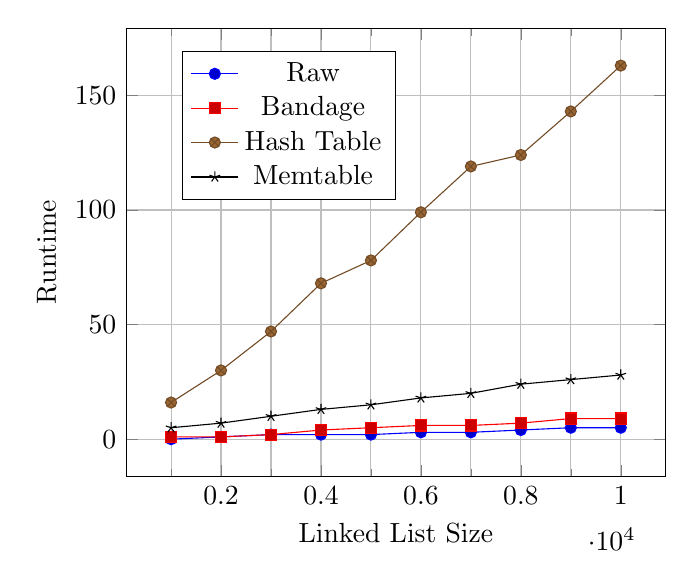
\begin{tikzpicture}
  \begin{axis}[ 
      xlabel=Linked List Size,
      ylabel=Runtime,
      minor x tick num=1,
      grid=both,
	  legend style={at={(0.5,0.95)}}
    ] 
    \addplot coordinates{
		(	1000	,	0	)
		(	2000	,	1	)
		(	3000	,	2	)
		(	4000	,	2	)
		(	5000	,	2	)
		(	6000	,	3	)
		(	7000	,	3	)
		(	8000	,	4	)
		(	9000	,	5	)
		(	10000	,	5	)
    }; 
	\addlegendentry{Raw}
    \addplot coordinates{
		(	1000	,	1	)
		(	2000	,	1	)
		(	3000	,	2	)
		(	4000	,	4	)
		(	5000	,	5	)
		(	6000	,	6	)
		(	7000	,	6	)
		(	8000	,	7	)
		(	9000	,	9	)
		(	10000	,	9	)
    }; 
	\addlegendentry{Bandage}
    \addplot coordinates{
		(	1000	,	16	)
		(	2000	,	30	)
		(	3000	,	47	)
		(	4000	,	68	)
		(	5000	,	78	)
		(	6000	,	99	)
		(	7000	,	119	)
		(	8000	,	124	)
		(	9000	,	143	)
		(	10000	,	163	)
	}; 
	\addlegendentry{Hash Table}
    \addplot coordinates{
		(	1000	,	5	)
		(	2000	,	7	)
		(	3000	,	10	)
		(	4000	,	13	)
		(	5000	,	15	)
		(	6000	,	18	)
		(	7000	,	20	)
		(	8000	,	24	)
		(	9000	,	26	)
		(	10000	,	28	)
	}; 
	\addlegendentry{Memtable}
  \end{axis}
\end{tikzpicture}
\caption{Increase in runtime following a Linked List as size increases}
\label{fig:LinkedListScaling}
\end{figure}


Figure \ref{fig:LinkedListScaling} shows the results.
The first and most obvious result is that, now that the pointers are stored on the heap and therefore table lookups are required for pointer bounds the table lookup approaches are slower than the fat pointer approach.

The hash table performs the worst with a \verb!32x! runtime increase at the largest list size.
This is not surprising considering that each lookup requires a look through each bucket for the matching element.
The interesting result is that the runtime seems to increase linearly with the list size, implying a close to $O(1)$ overhead for hashtable lookup.

With the longest linked list length, the MemTable takes five times as long as with no bounds checking and three times longer than bandage.
The MemTable lookup consists of pointer arithmetic and an access to the \verb!mmap!ed area, whereas a fat pointer lookup consists of a \verb!GEP! to the object.
A potential reason the MemTable approach takes longer than fat pointers is that an iteration for the fat pointer contains a load which fetches both the next pointer value and its bound at the same time, and they are store contiguously in memory.
An iteration with MemTables consists of a lookup to find the next pointer, and then a lookup in the table to find the bounds for that pointer, requiring two lookups to two areas of memory that are likely very far apart.

However, since the linked list was allocated in order, each element is likely arranged sequentially in memory.
Therefore, since the MemTable uses the pointer's address in memory as the index to that pointer's information, the bounds information associated with each linked list item will also be arranged sequentially in memory, and quite close together, giving very good spatial locality for the caches to take advantage of.

A final cause of the slowdown could be that since the table lookup functions are compiled separately and linked with the code that uses them it prevents them from being inlined, resulting in more jumping around.
 linear

\subsection{Olden Benchmarks}

The olden suite of benchmarks are designed to be very pointer operation heavy.

\subsubsection{Treeadd}

The treeadd benchmark constructs a binary tree where each node contains a value in addition to two children (all values are set to 1).
A depth-first search is then performed, accumulating the value at each node.

The implementation of CCured-like analysis counts all member pointers as a non-SAFE type (since the actions on the pointer and therefore the CCured type will be different for each instance), meaning that the tree traversal doesn't benefit from CCured-analysis.

Under Bandage, the tree construction stage, dominated by memory allocations took a \verb!42%! performance hit and the tree traversal stage took a \verb!77%! performance hit.

% 744809 223446 968255
% 1060893 395186 1456079
% Unoptimized bounds checking

\subsubsection{Bisort}

The bisort benchmark constructs a binary tree with each node containing a random value.
The tree is then sorted by performing a binary merge at each node, working up to the root node.

Under Bandage, tree construction displayed little overhead with a \verb!3%! slowdown, though the sorting caused a larger overhead of \verb!165%!, resulting in an overall runtime increase of \verb!83%!.

\subsubsection{Mst}
\subsubsection{Perimeter}
\verb!-8%!
\verb!23%!
\verb!-3%!
\subsubsection{Power}
\subsubsection{Tsp}

The tsp benchmark constructs a 2d tree of nodes and proceeds to solve the travelling salesman problem.
For nodes close together, it uses the closest pointer heuristic.

Under Bandage, tree construction introduced no overhead but application of the travelling salesman problem increased runtime by \verb!103%!.

\subsubsection{Other Benchmarks}

Due to the complex nature of the transformation (especially the fat pointer transformation), some of the olden benchmarks are not transformed correctly.

%\subsubsection{Type Coercion}

One of reasons that the benchmarks fail to run is Type Coercion.
In some circumstances, the LLVM IR produced by clang coerces the types of parameters to functions.
For example, the \verb!em3d! benchmark contains the following function:

\begin{minted}[frame=single]{c}
typedef struct node_t{
    double value;
} node_t;

typedef struct graph_t{
    node_t *e;
    node_t *h;
} graph_t;

void print_graph(graph_t graph){...}
\end{minted}

Instead of the struct being passed to the function as a whole struct, it is split into its two members and the function in IR actually takes two \verb!node_t *!s as its parameters, which are then put into a anonymous type of \verb!{node_t *, node_t *}! which is finally bitcast into a \verb!graph_t!.

\subsection{No Checks}

Bandage was modified to not insert bounds or null checks on pointer dereference, and the benchmarks were run again.
This provided a measurement of the overhead introduced by using fat pointers (and therefore dealing with the extra loads, pointer wrapping and stripping and cache overhead) and by propegating the bounds information.
The overheads introduced here allow evaluation of the bounds checking strategy separate from those overheads and also provides a theoretical lower bound on what an optimization to the checking strategy can achieve.

\begin{table}
\centering
\begin{tabular}{|l|r|r|}
\hline \textbf{Olden Benchmark} & \textbf{O0 Overhead} & \textbf{O3 Overhead}\\
\hline Bisort       &   7.50\%   &   3.44\% \\
\hline Mst          & xxxxxx\%   & xxxxxx\% \\
\hline Perimeter    & -18.62\%   & -43.49\% \\
\hline Power        & xxxxxx\%   & xxxxxx\% \\
\hline Treeadd      &  28.75\%   &  17.11\% \\
\hline Tsp          &   7.29\%   &  28.57\% \\
\hline
\end{tabular}
\caption{Runtime overhead on olden benchmarks when no bounds or null checks are inserted}
\label{tab:NoChecks}
\end{table}

The runtime overheads are shown in Table \ref{tab:NoChecks}, for comparison when the code was run without optimization and when the code was run with O3.
It is gratifying to see that in most of the cases, O3 optimization reduces the gap between uninstrumented and instrumented code.

\subsubsection{Tsp interfering with Optimization}

Looking at the runtime breakdown of the Tsp benchmark gives us the timings in Table \ref{tab:TspNoChecks}.
It can be seen that large discrepancy in optimization speedups arises during the set of O1 optimizations.

\begin{table}
\centering
\begin{tabular}{|l|r|r|}
\hline  \textbf{Optimization Level}  &   \textbf{Raw} &   \textbf{Bandage} \\
\hline  O1  &   20.51\%  &   -2.33\%  \\
\hline  O2  &   26.92\%  &   13.95\%  \\
\hline  O3  &   26.92\%  &   13.95\%  \\
\hline
\end{tabular}
\caption{Speedup relative to O0 optimization for raw and bandage transformed Tsp benchmark.}
\label{tab:TspNoChecks}
\end{table}

In order to investigate this further, O1 optimization was repeated multiple times on the uninstrumented code, each time with a specific optimization disabled, to determine which was responsible for the \verb!20%! speedup.
Each of the resulting binaries displayed speedups of \verb!17%! or more, suggesting that no single optimization was responsible for the speedup.
It was found however, when the \verb!instcombine! optimization was omitted, the speedup for the unoptimized binary was \verb!25%!, indicating that it actually slows the resulting program.

The same process was repeated on the instrumented IR.
It was found that with each optimization pass specified manually, a speedup of \verb!25\%! is achieved - similar to that of the raw binary, but when specified through the O1 flag, the speedup is negligable.

However, this process also identified the O1 optimizations that were the most responsible for was responsible for the speedup.
Without the \verb!instcombine! or the \verb!sroa! optimizations, the speedup dropped to \verb!1%!.
Additionally, the absence of the \verb!early-cse! optimization caused the speedup to drop to \verb!17%!.

\section{Interactions with Optimizations passes}

It was seen in the previous section that there were three O1 optimizations that produced significant changes in the runtime of the instrumented code.

\section{Security}

\subsection{Buffer Overflow Attack}

\begin{minted}[frame=single]{c}
int main(void){
    char pass[16];
    int userid = 0;

    gets(pass);
    ...
}
\end{minted}

\begin{minted}[frame=single]{c}
// In stdio
char *gets(char *buf)
{
    int c;
    char *s;
    for (s = buf; (c = getchar()) != '\n';)
        if (c == EOF)
            if (s == buf)
                return (NULL);
            else
                break;
        else
            *s++ = c;
    *s = 0;
    return (buf);
}
\end{minted}
Bandage is capable of stopping the buffer overflow described in the Background section.
The \verb!pass! array has its bounds information contained in its type in LLVM IR (as \verb![16xi8]!).
As it is passed into \verb!gets! as a parameter it is converted into a function whose value is set to the address of the array.
During the assignment, the bounds of the fat pointer are set correctly.
Then as \verb!s! is set to \verb!buf!, the bounds information is transferred to \verb!s! and consulted on every dereference of \verb!s!.
Therefore once the value of \verb!s! exceeds its base and bounds (that of the original variable \verb!pass!) an error is triggered.

\subsection{Heartbleed}

\begin{minted}[frame=single]{c}
/* Read type and payload length first */
hbtype = *p++;
n2s(p, payload);
pl = p;
...
unsigned char *buffer, *bp;
int r;

buffer = OPENSSL_malloc(1 + 2 + payload + padding);
bp = buffer;
...
/* Enter response type, length and copy payload */
*bp++ = TLS1_HB_RESPONSE;
s2n(payload, bp);
memcpy(bp, pl, payload);
\end{minted}


%\section{Misc}
%\subsection{Fat Pointers}

%Fat pointers add a storage overhead in the pointer itself, tripling its size to that of three pointers.
%Fat pointers generate computational overhead on creation, where the base and bound must be set as well as the value and on dereference, where an extra load instruction must be added.
%Finally fat pointers create computational overhead on bounds checking.

%\subsection{Fat Pointers with CCured Analysis}

%\subsubsection{Safe pointers as Raw or Fat Pointers}

%When combining the CCured approach with the fat pointer analysis, there is a choice of how to implement pointers designated as SAFE - these are pointers that do not require bounds checks on dereference.
%These SAFE pointers can either be implemented as a fat pointer but without bounds checking or kept as a raw pointer.

%Implementing SAFE pointers as fat pointers but without the bounds checking brings consistency but keeps the overhead of fat pointers, which isn't used when SAFE pointers are kept as raw pointers.
\subsection{Returning a Local Variable}

\begin{minted}[frame=single]{c}
int *ReturnLocalVariable(){
    int x = 5;
    return &x;
}
int main(){
    int *a = ReturnLocalVariable();
    *a = 12;
    return 0;
}
\end{minted}

Bandage, a system for enforcing spatial pointer safety cannot detect what is wrong with this example of a temporal pointer violation.
The expression \verb!&x! is turned into a fat pointer, with value and base pointing to the address of \verb!x! and the bound pointing past its end.
After return, it is still a perfectly valid fat pointer as the value is within the base and bound.
Therefore on dereference, no error is triggered.


\chapter{Summary and Conclusions} 

The novel idea of separation of analysis and implementation was developed and implemented paving the way for a reusable ecosystem of components to enforce pointer safety and to identify where it needs to be enforced.

The two prevalent methods of carrying spatial pointer information and tracking its safety were implemented and their effects on commonly used compiler optimizations was investigated.
\textbf{It was found that...}

By placing the existing pointer safety systems in a common evaluation framework they can be compared and contrasted, allowing the users to make a choice of which system to use or allowing researchers to identify gaps in the design space for future work.
This evaluation also identified a core trade-off in this area, that of compatibility vs completeness, with Cyclone taking its place at the completeness end of the spectrum and Heapmon taking its place at the compatibility end.

\section{Software Engineering Practices}

The use of a strong test suite was invaluable during the implementation, and the only thing I would change if I did this again would be making it even stronger.

In terms of implementation costs, implementing Bandage took considerably more effort and was far more bug prone than implementing SoftBound.
This is in large part due to Bandage changing the representation of pointers - making the change from raw pointers to fat pointers required a considerable amount of code to be written in one piece - if the entire change did not work, the source programs would break.
In the SoftBound implementation however, the implementation could be broken down into small pieces (eg providing bounds for local variables, then passing them through functions), and at each stage the source programs would compile, though the checking may not be complete.

Although this does provide a nice guarantee with Bandage that if the program compiles, bounds checking is more likely to be thorough, it creates an all-or-nothing situation in the presence of cases that haven't been implemented where Bandage either breaks the code or performs well, while Softbound can provide bounds checking for that that has been implemented.

Unexpected setbacks were discovered in trying to run the Softbound transformation on the Raspberry Pi, as both uthash and memtables required modification to run on 32-bit systems.

\appendix
\singlespacing

\bibliographystyle{plain} 
\bibliography{Bibliography} 

\end{document}
